\documentclass[a4paper]{article}
\usepackage{standalone}

\usepackage{color}
\usepackage{url}
\usepackage[T2A]{fontenc} % enable Cyrillic fonts
\usepackage[utf8]{inputenc} % make weird characters work
\usepackage{graphicx}
\usepackage[table,xcdraw]{xcolor}
\graphicspath{ {./Slike/} }
\usepackage{float}
\restylefloat{table}

\usepackage[english,serbian]{babel}
%\usepackage[english,serbianc]{babel} %ukljuciti babel sa ovim opcijama, umesto gornjim, ukoliko se koristi cirilica

\usepackage[unicode]{hyperref}
\hypersetup{colorlinks,citecolor=green,filecolor=green,linkcolor=blue,urlcolor=blue}

\usepackage{listings}
%\usepackage{xurl}
\usepackage{pifont}

%\newtheorem{primer}{Пример}[section] %ćirilični primer
\newtheorem{primer}{Primer}[section]


\definecolor{mygreen}{rgb}{0,0.6,0}
\definecolor{mygray}{rgb}{0.5,0.5,0.5}
\definecolor{mymauve}{rgb}{0.58,0,0.82}

\lstset{ 
  backgroundcolor=\color{white},   % choose the background color; you must add \usepackage{color} or \usepackage{xcolor}; should come as last argument
  basicstyle=\scriptsize\ttfamily,        % the size of the fonts that are used for the code
  breakatwhitespace=false,         % sets if automatic breaks should only happen at whitespace
  breaklines=true,                 % sets automatic line breaking
  captionpos=b,                    % sets the caption-position to bottom
  commentstyle=\color{mygreen},    % comment style
  deletekeywords={...},            % if you want to delete keywords from the given language
  escapeinside={\%*}{*)},          % if you want to add LaTeX within your code
  extendedchars=true,              % lets you use non-ASCII characters; for 8-bits encodings only, does not work with UTF-8
  firstnumber=1,                % start line enumeration with line 1000
  frame=single,	                   % adds a frame around the code
  keepspaces=true,                 % keeps spaces in text, useful for keeping indentation of code (possibly needs columns=flexible)
  keywordstyle=\color{blue},       % keyword style
  language=C++,                 % the language of the code
  morekeywords={*,...},            % if you want to add more keywords to the set
  numbers=left,                    % where to put the line-numbers; possible values are (none, left, right)
  numbersep=5pt,                   % how far the line-numbers are from the code
  numberstyle=\tiny\color{mygray}, % the style that is used for the line-numbers
  rulecolor=\color{black},         % if not set, the frame-color may be changed on line-breaks within not-black text (e.g. comments (green here))
  showspaces=false,                % show spaces everywhere adding particular underscores; it overrides 'showstringspaces'
  showstringspaces=false,          % underline spaces within strings only
  showtabs=false,                  % show tabs within strings adding particular underscores
  stepnumber=1,                    % the step between two line-numbers. If it's 1, each line will be numbered
  stringstyle=\color{mymauve},     % string literal style
  tabsize=2,	                   % sets default tabsize to 2 spaces
  title=\lstname                   % show the filename of files included with \lstinputlisting; also try caption instead of title
}

\addtocontents{toc}{\setcounter{tocdepth}{1}} 

\begin{document}

\documentclass{article}
\begin{document}
\title{Informacioni sistem banke\\ \small{Seminarski rad u okviru kursa\\Informacioni sistemi\\ Matematički fakultet}}
\author{\\
Ivana Cvetkoski
\\
Bojana Ristanović
\\
Nikola Stamenić
}

\end{document}

\maketitle
\newpage

\section{Slučajevi upotrebe}
\documentclass{article}
\usepackage[pdftex]{graphicx}  
\begin{document}
\subsection{\bfseries Otvaranje računa}
\begin{figure}
\begin{center}
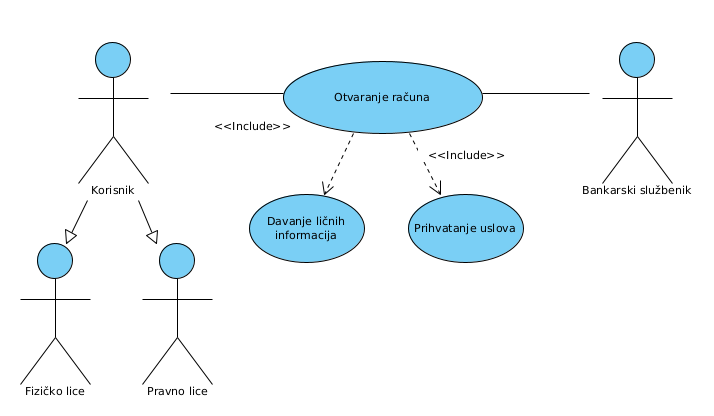
\includegraphics[scale=0.5]{./UseCases/Pictures/otvaranjeRacuna.png}
\end{center}
    \caption{Dijagram slučaja upotrebe otvaranja računa korisnika.}
\label{fig:Otvaranje računa}
\end{figure}


\subsubsection{ Otvaranje računa}

\begin{itemize}
    \item Kratak opis:
        \begin{itemize}
            \item Korisnik otvara račun u banci kako bi mogao da koristi pogodnosti koje ona nudi.
        \end{itemize}
    \item Učesnici:
        \begin{itemize}
            \item Zainteresovana osoba koja želi da ima račun u banci.
            \item Službeno lice koje je zaposleno u banci.
        \end{itemize}
    \item Preduslovi:
        \begin{itemize}
            \item Korisnik mora da bude punoletan.
            \item Korisnik mora da priloži tačne informacije.
            \item Korisnik mora da ima važeću ličnu kartu.
            \item Sistem mora biti u funkciji.
            \item Službeno lice mora biti autorizovano za korišćenje sistema.
        \end{itemize}
    \item Postuslovi:
        \begin{itemize}
            \item Korisnik je registrovan i ima otvoren račun u banci.
            \item Korisnik je ubačen u bazu podataka.
            \item Aktivirana je izrada korisnikove kartice.
        \end{itemize}
    \item Glavni tok:
        \begin{enumerate}
            \item Korisnik dolazi u filijalu i razgovara sa bankarskim službenikom.
            \item Bankarski službenik bira opciju za otvaranje novog računa.
            \item Sistem izbacuje formular.
            \item Službeno lice traži ličnu korisniku kartu.
            \item Korisnik prilaže ličnu kartu.
            \item Službeno lice popunjava u formularnu JMBG korisnika.
            \item Bankarski službenik ispituje korisnika o ostalim potrebnim informacijama.
            \item Korisnik daje tražene informacije.
            \begin{enumerate}
                \item Ukoliko je korisnik fizičko lice izvršava se podtok P1.
                \item Ukoliko je korisnik pravno lice izvršava se podtok P2.
            \end{enumerate}
            \item Službeno lice daje ugovor korisniku sa uslovima korišćenja računa u banci.
            \item Korisnik čita i prihvata uslove (potpisuje ugovor).
            \item Službenik unosi informacije u sistem i potvrdjuje unos.
            \item Sistem vrši validaciju podataka.
            \item Sistem čuva podatke.
            \item Bankarski službenik obaveštava korisnika da je račun aktiviran.
        \end{enumerate}
    \item Podtokovi:
        P1 Korisnik je fizičko lice:
        \begin{itemize}
            \item Ukoliko korisnik otvara račun kako bi primao platu mora dati podatke o firmi u kojoj radi.
        \end{itemize}   
        P2 Korisnik je pravno lice:
        \begin{itemize}
            \item Korisnik dostavlja rešenje o otvaranju firme (vlasnik firme, PIB, matični broj firme..) i karton deponovanih potpisa.
            \item Službeno lice izvlači rešenje o otvaranju firme iz APR-a.
            \item Službeno lice vrši proveru informacija tako što uporedjuje korisnikove i podatke iz APR-a.
            \item Službeno lice otvara novi formular i popunjava polja sa dostavljenim podacima.
            \item Službeno lice potvrdjuje unos u formularu.
            \item Služba za kontrolu dokumentacije pravnih lica vrši proveru unetih informacija.
            \item Unete informacije se čuvaju u sistemu.
        \end{itemize}    
    \item Alternativni tok:
        \begin{itemize}
            \item Prilikom 10. koraka glavnog toka korisnik odbija uslove otvaranja računa. Bankarski službenik poništava sve što je uneo u formular i svi podaci se brišu.
            \item Prilikom 12. koraka može doći do neuspešne validacije podataka, u tom slučaju sistem će izbaciti obaveštenje i biće onemogućeno čuvanje podataka dok se ne ispravi propust.
        \end{itemize}
    \item Dodatne informacije:
        \begin{itemize}
            \item Uslovi otvaranja računa u banci su regulisani zakonom. Nepoštovanje tih uslova može dovesti do sudskih postupaka.
        \end{itemize}
\end{itemize}

\end{document}

\documentclass{article}
\begin{document}
Transakcije

\end{document}

\documentclass{article}
\begin{document}

\subsection{Proizvodi}

Proizvodi predstavljaju slučaj upotrebe u kom se formalizuju usluge koje banka pruža korisnicima. Potrebno je da korisnik podnese zahtev banci za korišćenje određenog proizvoda (lično u banci ili popunjavanjem forme putem online bankarstva). Zahtevi se obrađuju i ako ih banka odobri, korisniku je omoguceno koriscenje proizvoda.

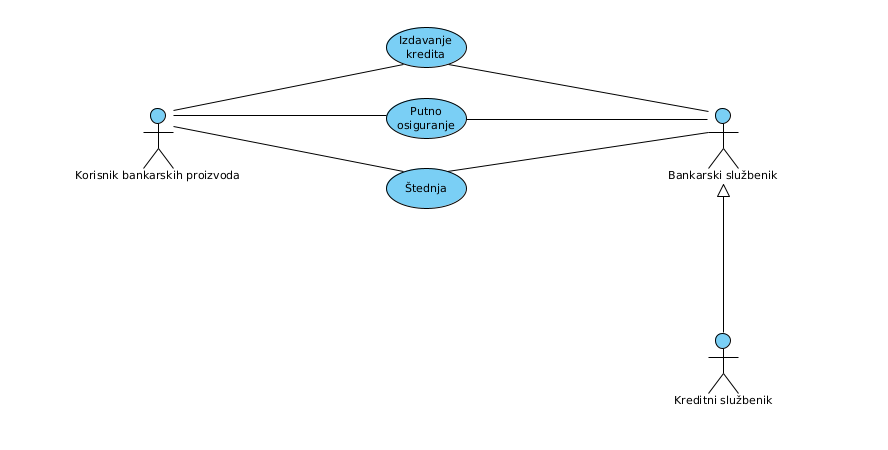
\includegraphics[scale = 0.4]{./UseCases/Pictures/Bank_products.png}

\subsubsection{Slucaj upotrebe: Izdavanje kredita}

Kratki opis: Korisnik šalje zahtev za otvaranje kredita. Banka proverara korisnika, otvara mu račun (ukoliko korisnik već nema otvoren račun u toj banci) i uplaćuje željeni iznos.\\
Učesnici: 
\begin{enumerate}
\item Kreditno odeljenje - kreditni službenik
\item Korisnik proizvda banke
\end{enumerate}
Preduslovi: 
\begin{enumerate}
\item Banka ima u ponudi zahtevani proizvod korisnika
\item Korisnik ima preko 24 godine i u stalnom je radnm odnosu duze od 3 meseca 
\item Zahtev je uspešno dostavljen kreditnom odeljenju za njegovu obradu 
\end{enumerate}
Postuslovi: 
\begin{enumerate}
\item Korisniku je otvoren racun u banci na kom se nalazi zahtevani iznos kredita 
\item Korisniku je uručen plan otplate kredita. 
\end{enumerate}
Glavni tok: 
\begin{enumerate}
\item Korisnik na uvid donosi ličnu kartu 
\item Kreditni službenik (bankar) u sistem unosi zahtev za podizanje kredita 
\item Korisnik od bankara dobija obrazac koji je potrebno da overi u firmi u kojoj je zaposlen 
\item Bankar podatke o firmi unosi u sistem banke 
\item Ovlašćeni radnik banke dobija izveštaj o korisniku od Kreditnog biroa 
\item Kreditno odeljenje banke treba da ustanovi da li je moguce korisniku izdati kredit u željenom iznosu 
\item Ukoliko su svi uslovi ispunjeni, korisnik potpisuje ugovor i menicu 
\end{enumerate}
\end{document}


\end{document}
